
% v2-acmsmall-sample.tex, dated March 6 2012
% This is a sample file for ACM small trim journals
%
% Compilation using 'acmsmall.cls' - version 1.3 (March 2012), Aptara Inc.
% (c) 2010 Association for Computing Machinery (ACM)
%
% Questions/Suggestions/Feedback should be addressed to => "acmtexsupport@aptaracorp.com".
% Users can also go through the FAQs available on the journal's submission webpage.
%
% Steps to compile: latex, bibtex, latex latex
%
% For tracking purposes => this is v1.3 - March 2012
\documentclass[prodmode,acmtecs]{acmsmall} % Aptara syntax
\usepackage[spanish,polish]{babel}
\usepackage[T1]{fontenc}
\usepackage{fancyvrb}
\usepackage{graphicx,hyperref}
\newcommand\cutout[1]{}


\usepackage[table]{xcolor}
\usepackage[utf8]{inputenc}
\usepackage[parfill]{parskip}
\usepackage{tabulary}
\PassOptionsToPackage{hyphens}{url}
\usepackage{hyperref}    
\usepackage[capitalize]{cleveref}


% Metadata Information
% !!! TODO: SET THESE VALUES !!!
\acmVolume{0}
\acmNumber{0}
\acmArticle{CFP}
\acmYear{0}
\acmMonth{0}

\newcounter{colstart}
\setcounter{page}{4}

\RecustomVerbatimCommand{\VerbatimInput}{VerbatimInput}%
{
%fontsize=\footnotesize,
fontfamily=\rmdefault
}


\newcommand{\UnderscoreCommands}{%\do\verbatiminput%
\do\citeNP \do\citeA \do\citeANP \do\citeN \do\shortcite%
\do\shortciteNP \do\shortciteA \do\shortciteANP \do\shortciteN%
\do\citeyear \do\citeyearNP%
}

\usepackage[strings]{underscore}



% Document starts
\begin{document}


\setcounter{colstart}{\thepage}

\acmArticle{CFP}
\title{\huge\sc SIGLOG Monthly 211}
\author{DAVID PURSER\affil{Max Planck Institute for Software Systems, Saarbr\"ucken}
\vspace*{-2.6cm}\begin{flushright}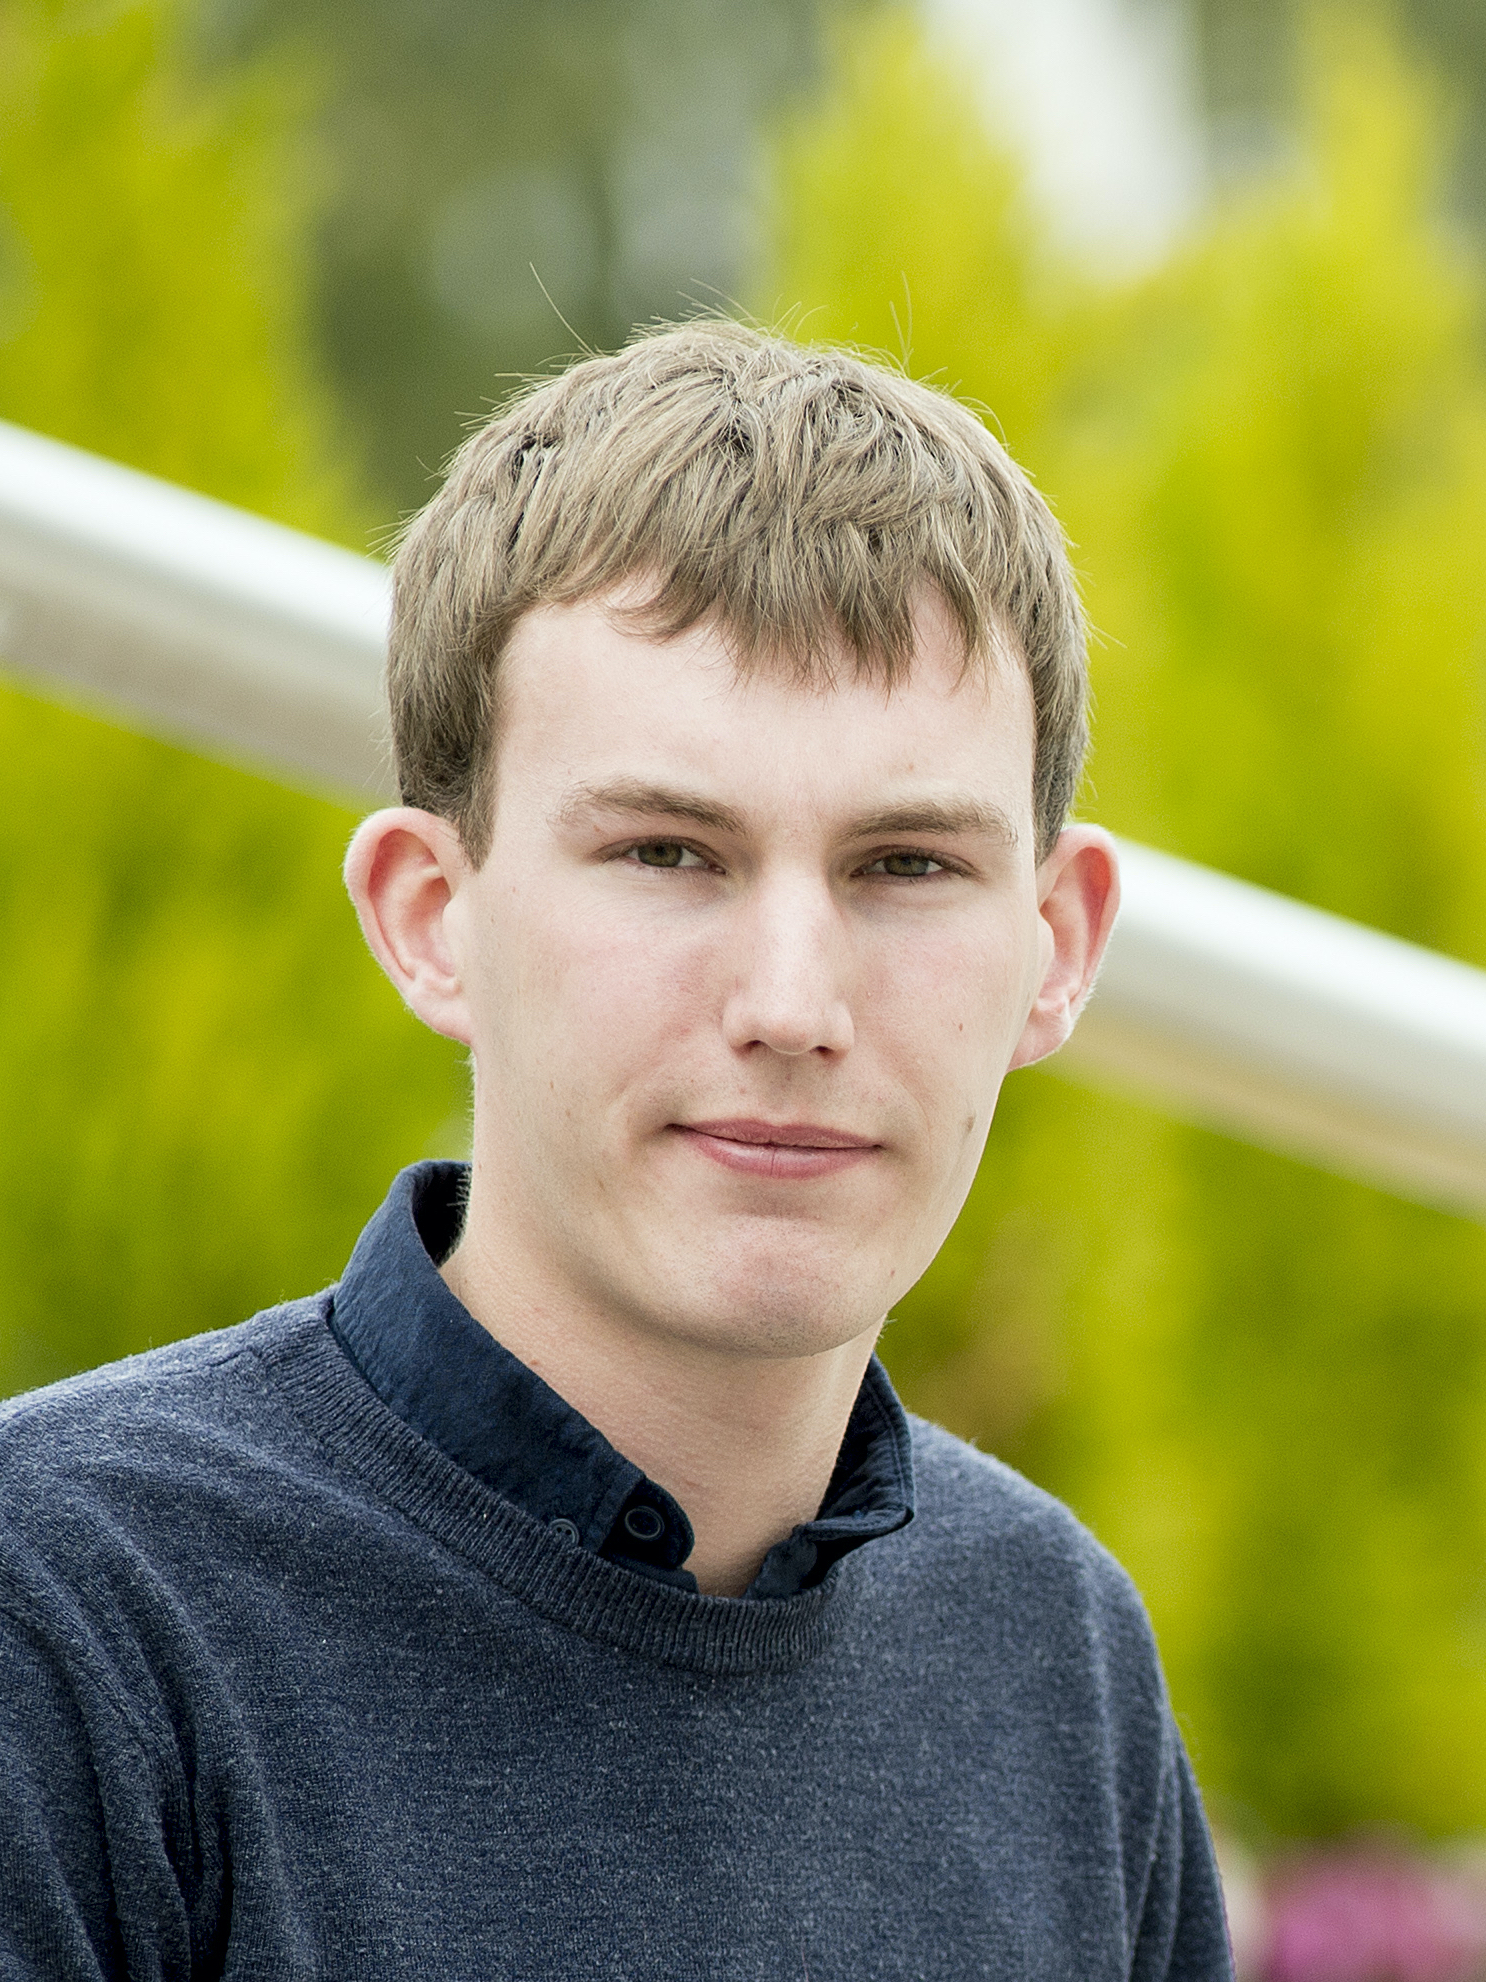
\includegraphics[width=30mm]{dp}\end{flushright}
}

\maketitlee

\href{https://lics.siglog.org/newsletters/}{Past Issues}
 - 
\href{https://lics.siglog.org/newsletters/inst.html}{How to submit an announcement}
\section{Table of Content}\begin{itemize}\item DEADLINES (\cref{deadlines}) 
 
\item COVID UPDATES 
 
\begin{itemize}\item LICS 2021 (\cref{LICS2021})
\end{itemize} 
\item CALLS 
 
\begin{itemize}\item SOAP (CALL FOR PAPERS) (\cref{SOAP})
\item MGS 21 (CALL FOR PARTICIPATION) (\cref{MGS21})
\item CONCUR 2021 (CALL FOR PAPERS) (\cref{CONCUR2021})
\item ICGI 2020/21 (CALL FOR PAPERS) (\cref{ICGI202021})
\item ACKERMANN AWARD 2021 (CALL FOR NOMINATIONS) (\cref{ACKERMANNAWARD2021})
\item CSL22 (CALL FOR PAPERS) (\cref{CSL22})
\end{itemize} 
\end{itemize}\section{Deadlines}\label{deadlines}\rowcolors{1}{white}{gray!25}\begin{tabulary}{\linewidth}{LL}SPIN 2021:  & Mar 1, 2021 (Paper) \\
Alonzo Church Award:  & Mar 1, 2021 (Deadline for Nominations) \\
QPL 2021:  & Mar 12, 2021 (Paper deadline (extended)) \\
TARK 2021:  & Mar 15, 2021 (Abstract), Mar 20, 2021 (Extended abstract) \\
SOAP:  & Mar 22, 2021 (Paper) \\
NALOMA'21:  & Mar 26, 2021 (Papers \& extended abstracts) \\
Diagrams 2021:  & Apr 01, 2021 (Titles+short abstracts), Apr 08, 2021 (Long and Short Papers), Apr 15, 2021 (Abstracts and Posters) \\
MGS 21:  & Apr 01, 2021 (Registration deadline) \\
FORMATS 2021:  & Apr 06, 2021 (Abstract), Apr 13, 2021 (Paper) \\
E. W. Beth Outstanding Dissertation Prize 2021:  & Apr 15, 2021 (Deadline for nominations) \\
CONCUR 2021:  & Apr 23, 2021 (Abstract), Apr 30, 2021 (Paper) \\
MFCS 2021:  & Apr 30, 2021 (Abstract), May 03, 2021 (Paper) \\
ICGI 2020/21:  & May 25, 2021 (Paper) \\
ACKERMANN AWARD 2021:  & Jul 01, 2021 (Deadline for nomination) \\
CSL22:  & Jul 05, 2021 (Abstract), Jul 12, 2021 (Paper) \\
\end{tabulary}
\section{LICS 2021:}\label{LICS2021}COVID UPDATE 

\begin{itemize}\item  LICS 2021 will be online only. 
 
\end{itemize}\section{SOAP: The 10th ACM SIGPLAN International Workshop on the State of the Art in Program Analysis }\label{SOAP}  Co-located with PLDI 2021\\ 
  June 2021 - Virtual\\ 
  \href{https://pldi21.sigplan.org/home/SOAP-2021}{https://pldi21.sigplan.org/home/SOAP-2021}\\ 
  \href{https://twitter.com/SOAP_Workshop}{https://twitter.com/SOAP\_Workshop}\\ 
CALL FOR PAPERS 

\begin{itemize}\item  Static and dynamic analysis techniques and tools for Java, and other programming languages, have received widespread attention for a long time. The application domains of these analyses range from core libraries to modern technologies such as web services and Android applications. Over time, various analysis frameworks have been developed to provide techniques for optimizing programs, ensuring code quality, and assessing security and compliance. 
 
  SOAP 2021 aims to bring together the members of the program analysis community to share new developments and shape new innovations in program analysis. For SOAP 2021, we invite contributions and inspirations from researchers and practitioners working with program analysis. We are particularly interested in exciting analysis framework ideas, innovative designs, and analysis techniques, including preliminary results of work in progress. We will also focus on the state of the practice for program analysis by encouraging submissions by industrial participants, including tool demonstration submissions. The workshop agenda will continue its tradition of lively discussions on extensions of existing frameworks, development of new analyses and tools, and how program analysis is used in real-world scenarios. 
 
\item  Possible submissions include, but are not limited to: 
 
\begin{itemize}\item  A report on a novel implementation of a program analysis, with a focus on practical details or optimization techniques for obtaining precision and performance.
\item  A new research tool, data, and other artifacts, that showcase early implementations of novel program analysis concepts, as well as mature prototypes.
\item  A description of a new analysis component, for example, front-ends or abstract domains.
\item  A report describing an innovative tool built on top of an existing framework.
\item  A compelling use case for a feature that is not yet supported by existing analysis tools, with good examples and an informal design of the proposed feature.
\item  An idea paper proposing the integration of existing program analyses to answer interesting novel questions about programs, for example in IDEs.
\item  An experience report on the use of a program analysis framework.
\item  A description of a program analysis tool and screenshots of main parts of the demo.
\end{itemize} 
\item  SUBMISSIONS  
 
  Submissions should be four to six-page papers and should be formatted according to the two-column ACM proceedings format (\href{http://www.sigplan.org/Resources/Author}{http://www.sigplan.org/Resources/Author}). Each reference must list all authors of the paper. The citations should be in numerical style, e.g., [52]. The preprint template should be set to use 10pt font and ‘numbers’ to ensure numerical style citations, that is: \textbackslash{}documentclass[10pt, numbers]\{sigplanconf\}.  
 
  Submissions should be made on EasyChair: \href{https://easychair.org/conferences/?conf=soap2021}{https://easychair.org/conferences/?conf=soap2021} 
 
\item  IMPORTANT DATES 
 
\rowcolors{1}{white}{gray!25}\begin{tabulary}{\linewidth}{LL}Paper submission:  & Mar 22, 2021 \\
Author notification:  & Apr 20, 2021 \\
Camera ready deadline:  & May 03, 2021 \\
\end{tabulary}
 
\item  CONTACT:  
 
  Contact the chairs Lisa Nguyen Quang Do nqd.lisa@gmail.com and Caterina Urban caterina.urban@inria.fr and follow @SOAP\_Workshop on Twitter. 
 
\end{itemize}\section{MGS 21: 21st Midlands Graduate School in the Foundations of Computing Science}\label{MGS21}  12-16 April 2021, virtually\\ 
  \href{https://staffwww.dcs.shef.ac.uk/people/G.Struth/mgs21.html}{https://staffwww.dcs.shef.ac.uk/people/G.Struth/mgs21.html}\\ 
CALL FOR PARTICIPATION 

\begin{itemize}\item  OVERVIEW  
 
  The annual Midlands Graduate School in the Foundations of Computing Science (MGS) offers an intensive programme of lectures on the mathematical foundations of computing. It addresses first of all PhD students in their first or second year, but is open to anyone interested in its topics, from academia to industry and around the world. The MGS has been run since 1999 and is hosted alternately by the Universities of Birmingham, Leicester, Nottingham and Sheffield. MGS 21 is its 21st incarnation. Information about previous events can be found at the MGS web site: \href{http://www.cs.nott.ac.uk/MGS}{http://www.cs.nott.ac.uk/MGS} 
 
\item  PROGRAMME  
 
  MGS 21 consists of eight courses, each with four or five hours of lectures and a similar number of exercise sessions. Three courses are introductory; one is given by an invited lecturer. These should be attended by all participants. The remaining more advanced courses should be selected based on interest. MGS 21 aims at a mix of livestreamed and prerecorded lectures and livestreamed exercise sessions, with additional social online events. 
 
\item  INVITED LECTURES:  
 
\begin{itemize}\item  Monads and Interactions, Tarmo Uustalu, Reykjavik
\end{itemize} 
  Introductory courses: 
 
\begin{itemize}\item  Category Theory, Jacopo Emmenegger, Birmingham
\item  Type Theory, Thorsten Altenkirch, Nottingham
\item  Proof Theory, Anupam Das, Birmingham
\end{itemize} 
  Advanced courses: 
 
\begin{itemize}\item  Homotopy Type Theory, Nicolai Kraus, Nottingham
\item  Inductive and Coinductive Reasoning with Isabelle/HOL, Andrei Popescu, Seffield
\item  Effects and Call-by-Push-Value, Paul Levy, Birmingham
\item  Formal Modelling and Analysis of Concurrent Systems, Mohammad Mousavi, Licester
\end{itemize} 
  In addition we are organising a session where participants can briefly present and discuss their own research. A call will be made in March. 
 
\item  REGISTRATION 
 
  Participation at MGS 21 is free of charge, but selective. Requests must be submitted online via \href{https://staffwww.dcs.shef.ac.uk/people/G.Struth/mgs21.html}{https://staffwww.dcs.shef.ac.uk/people/G.Struth/mgs21.html} 
 
Registration deadline: Apr 01, 2021 
 
\item  ORGANISATION 
 
  Please direct all queries about MGS 21 to Georg Struth G.Struth@sheffield.ac.uk 
 
\end{itemize}\section{CONCUR 2021: The 32nd International Conference on Concurrency Theory}\label{CONCUR2021}  Aug 23-27, 2021, Online, Co-located with QUEST, FORMATS AND FMICS\\ 
  \href{https://qonfest2021.lacl.fr/}{https://qonfest2021.lacl.fr/}\\ 
CALL FOR PAPERS 

\begin{itemize}\item  The purpose of CONCUR 2021, the 32nd International Conference on Concurrency Theory, is to bring together researchers, developers, and students in order to advance the theory of concurrency, and promote its applications. 
 
  Due the pandemic situation, the organization committee decided that the conference will take place online as last year's CONCUR: the talks will be pre-recorded and then streamed on Zoom. The participants will be able to ask questions on Slack, and the speakers will answer them live during the online Zoom session. 
 
  Should the situation improve, and allow some international travel, we will be able to cater for a few people that would like to meet in person in Paris. 
 
\item  Invited Speakers: Patricia Bouyer-Decitre (ENS Paris Saclay), Davide Sangiorgi (University of Bologna), Boudewijn Haverkort (Tilburg University (Joint with QEST)) 
 
\item  IMPORTANT DATES (All dates are AoE). 
 
\rowcolors{1}{white}{gray!25}\begin{tabulary}{\linewidth}{LL}Abstract submission:  & Apr 23, 2021 \\
Paper submission:  & Apr 30, 2021 \\
Notification:  & Jun 23, 2021 \\
Camera ready copy:  & Jul 09, 2021 \\
Conference:  & Aug 23-27, 2021 \\
\end{tabulary}
 
\item  TOPICS 
 
  Submissions are solicited in semantics, logics, verification and analysis of concurrent systems. The principal topics include (but are not limited to):   
 
\begin{itemize}\item  Basic models of concurrency such as abstract machines, domain-theoretic models, game-theoretic models, process algebras, graph transformation systems, Petri nets, hybrid systems, mobile and collaborative systems, probabilistic systems, real-time systems, biology-inspired systems, and synchronous systems;
\item  Logics for concurrency such as modal logics, probabilistic and stochastic logics, temporal logics, and resource logics; 
\item  Verification and analysis techniques for concurrent systems such as abstract interpretation, atomicity checking, model checking, race detection, pre-order and equivalence checking, run-time verification, state-space exploration, static analysis, synthesis, testing, theorem proving, type systems, and security analysis;
\item  Distributed algorithms and data structures: design, analysis, complexity, correctness, fault tolerance, reliability, availability, consistency, self-organization, self-stabilization, protocols;
\item  Theoretical foundations of architectures, execution environments, and software development for concurrent systems such as geo-replicated systems, communication networks, multiprocessor and multi-core architectures, shared and transactional memory, resource management and awareness, compilers and tools for concurrent programming, programming models such as component-based, object- and service-oriented.
\end{itemize} 
\item  PAPER SUBMISSION 
 
  CONCUR 2021 solicits high quality papers reporting research results and/or experience related to the topics mentioned below. All papers must be original, unpublished, and not submitted for publication elsewhere. 
 
  Each paper will undergo a thorough review process. The paper may be supplemented with a clearly marked appendix, which will be reviewed at the discretion of the program committee.  
 
  Papers must be submitted in PDF format (LIPIcs style) via EasyChair and not exceed 14 pages (excluding references and clearly marked appendices). The CONCUR 2021 proceedings will be published by LIPIcs.  
 
\item  SPECIAL ISSUE 
 
  A special issue dedicated to selected papers from CONCUR 2021 will appear in Logical Methods in Computer Science. 
 
\item  TEST OF TIME AWARDS 
 
  Last year, the first CONCUR Test-of-Time awards were given. In 2021, the jury of the Test-of-Time award will consist of Rob van Glabbeek (chair), Luca de Alfaro, Nathalie Bertrand, Catuscia Palamidessi, and Nobuko Yoshida. The winners will be announced at the conference. 
 
\end{itemize}\section{ICGI 2020/21: THE 15TH INTERNATIONAL CONFERENCE ON GRAMMATICAL INFERENCE}\label{ICGI202021}  August 23-27, 2021, held online\\ 
  \href{https://icgi2020.lis-lab.fr}{https://icgi2020.lis-lab.fr}\\ 
CALL FOR PAPERS 

\begin{itemize}\item  It is our pleasure to inform you about ICGI 2020/21, the major forum for presentation and discussion of original research papers on all aspects of grammar learning. ICGI, which has been organized bi-annually since the early nineties, will be held on-line in August 2021 after being postponed due to COVID-19 last year. ICGI 2020/21 is the place to present your work on learning formal grammars, finite state machines, context-free grammars, Markov models, or any models related to language theory, stochastic or otherwise. Both theoretical work and experimental analyses are welcomed as submissions. This year we especially encourage submissions related to connectionist models such as neural networks, since there are tutorials scheduled on that topic.  
 
\item  The conference will be spread out over August 23-27, featuring a mix of live talks, asynchronous video presentations, tutorials, and an online competition. There will be one synchronous event per day plus dedicated time for each accepted paper; further details will be announced by email. 
 
\item  INVITED SPEAKERS:  
 
\begin{itemize}\item  Dana Fisman (Ben-Gurion University) 
\item  Robert Frank (Yale University) 
\item  Guillaume Rabusseau (Université de Montréal) 
\item  Gail Weiss (Technion - Israel Institute of Technology) 
\item  Others to be confirmed
\end{itemize} 
\item  ON-LINE COMPETITION 
 
 ICGI 2020/21 is hosting a shared task on morphological inflection. An example of English inflection is the conversion of the lemma ‘run’ to its present participle, ‘running’. To participate in the shared task, you will build a system that can learn to solve inflection problems. More details at \href{https://aryamccarthy.github.io/icgi2020/}{https://aryamccarthy.github.io/icgi2020/}  
 
\item  TOPICS OF INTEREST 
 
\begin{itemize}\item  Theoretical aspects of grammatical inference: learning paradigms, learnability results, complexity of learning;
\item  Empirical and theoretical research on query learning, active learning, and other interactive learning paradigms;
\item  Empirical and theoretical research on methods using or including, but not limited to, spectral learning, state-merging, distributional learning, statistical relational learning, statistical inference and/or Bayesian learning;
\item  Learning algorithms for language classes inside and outside the Chomsky hierarchy. Learning tree and graph grammars;
\item  Learning probability distributions over strings, trees or graphs, or transductions thereof;
\item  Learning with contextualized data: for instance, Grammatical inference from strings or trees paired with semantics representations, or learning by situated agents and robots;
\item  Experimental and theoretical analysis of different approaches to grammar induction, including artificial neural networks, statistical methods, symbolic methods, information-theoretic approaches, minimum description length, complexity-theoretic approaches, heuristic methods, etc;
\item  Novel approaches to grammatical inference: induction by DNA computing or quantum computing, evolutionary approaches, new representation spaces, etc;
\item  Successful applications of grammatical learning to tasks in fields including, but not limited to, natural language processing and computational linguistics, model checking and software verification, bioinformatics, robotic planning and control, and pattern recognition.
\end{itemize} 
\item  TYPES OF CONTRIBUTIONS 
 
\begin{itemize}\item  Formal and/or technical papers describe original solutions (theoretical, methodological or conceptual) in the field of grammatical inference. A technical paper should clearly describe the situation or problem tackled, the relevant state of the art, the position or solution suggested and the benefits of the contribution;
\item  Position papers can describe completely new research positions or approaches, open problems. Current limits can be discussed. In all cases rigor in presentation will be required. Such papers must describe precisely the situation, problem, or challenge addressed, and demonstrate how current methods, tools, ways of reasoning, may be inadequate;
\item  Tool papers describing a new tool for grammatical inference. The tool must be publicly available and the paper has to contain several use-case studies describing the use of the tool. In addition, the paper should clearly describe the implemented algorithms, input parameters and syntax, and the produced output.
\end{itemize} 
   Selected authors will be encouraged to submit an extended version of their work to an upcoming  special issue of an international journal (to be announced). 
 
\item  GUIDELINES FOR AUTHORS 
 
  Accepted papers will be published within the Proceedings of Machine Learning Research series (\href{http://proceedings.mlr.press/}{http://proceedings.mlr.press/}).  
 
  Max 12 pages, A4 pdf via EasyChair. JMLR style recommended (\href{https://ctan.org/tex-archive/macros/latex/contrib/jmlr}{https://ctan.org/tex-archive/macros/latex/contrib/jmlr}) since it will be the required format for the final published version. 
 
\item  Important Dates 
 
\rowcolors{1}{white}{gray!25}\begin{tabulary}{\linewidth}{LL}Paper submission:  & May 25, 2021 \\
Notification of acceptance:  & Jul 05, 2021 \\
Camera-ready copy:  & Jul 30, 2021 \\
Conference:  & Aug 23-27, 2021 \\
\end{tabulary}
 
\end{itemize}\section{ACKERMANN AWARD 2021: THE EACSL OUTSTANDING DISSERTATION AWARD FOR LOGIC IN COMPUTER SCIENCE}\label{ACKERMANNAWARD2021}  Deadline: 1 July 2021\\ 
CALL FOR NOMINATIONS 

\begin{itemize}\item  INTRODUCTION 
 
  Nominations are now invited for the 2021 Ackermann Award. 
 
\item  ELIGIBILITY 
 
  PhD dissertations in topics specified by the CSL and LICS conferences, which were formally accepted as PhD theses at a university or equivalent institution between 1 January 2019 and 31 December 2020 are eligible for nomination for the award. 
 
\item  PRESENTATION OF THE AWARD  
 
  The 2021 Ackermann award will be presented to the recipient(s) at CSL 2022, the annual conference of the EACSL.  The award consists of a certificate, an invitation to present the thesis at the CSL conference, the publication of the laudatio in the CSL proceedings, an invitation to the winner to publish thethesis in the FoLLI subseries of Springer LNCS, and  financial support to attend the conference. 
 
\item  JURY 
 
\begin{itemize}\item  Christel Baier (TU Dresden);
\item  Michael Benedikt (Oxford University);
\item  Mikolaj Bojanczyk (University of Warsaw);
\item  Jean Goubault-Larrecq (ENS Paris-Saclay);
\item  Prakash Panangaden (McGill University);
\item  Simona Ronchi Della Rocca (University of Torino), the vice-president of EACSL;
\item  Thomas Schwentick (TU Dortmund) , the president of EACSL;
\item  Alexandra Silva, (University College London), ACM SigLog representative.
\end{itemize} 
 The jury is entitled to give the award to more (or less) than one dissertation in a year. 
 
\item  WHAT TO SUBMIT 
 
  The candidate or his/her supervisor should submit 
 
\begin{itemize}\item  the thesis (ps or pdf file);
\item  a detailed description (not longer than 20 pages) of the thesis in ENGLISH (ps or pdf file);  it is recommended to not squeeze as much material as possible into these 20 pages, but rather to use them for a gentle introduction and overview, stressing the novel results obtained in the thesis and their impact;
\item  a supporting letter by the PhD advisor and two supporting letters by other senior researchers (in English); supporting letters can also be sent directly to Thomas Schwentick (thomas.schwentick@tu-dortmund.de);
\item  a short CV of the candidate;
\item  a copy of the document asserting that the thesis was accepted as a PhD thesis at a recognized University (or equivalent institution) and that the candidate has received his/her PhD within the specified period.
\end{itemize} 
\item  HOW TO SUBMIT 
 
  The submission should be sent by e-mail as attachments to the chairman of the jury, Thomas Schwentick: thomas.schwentick@tu-dortmund.de, with 
 
\begin{itemize}\item   Subject: Ackermann Award 2021 Submission
\item  Text: Name of candidate, list of attachments
\end{itemize} 
Deadline for nomination submission: Jul 01, 2021 
 
\end{itemize}\section{CSL22: Computer Science Logic}\label{CSL22}   February 14 - 19, 2022, in Göttingen, Germany (hybrid expected)\\ 
CALL FOR PAPERS 

\begin{itemize}\item  CONFERENCE 
 
  CSL is the annual conference of the European Association for Computer Science Logic (EACSL), see \href{https://www.eacsl.org/}{https://www.eacsl.org/}.  
 
  It is an interdisciplinary conference, spanning across both basic and application oriented research in mathematical logic and computer science.    
 
  Currently, we expect that the conference will be organized in a hybrid way: both with an in-presence component and an online component.  
 
\item  SUBMISSION GUIDELINES: 
 
  The CSL 2022 conference proceedings will be published in LIPIcs. Submitted papers must be in English and must provide sufficient detail to allow the Programme Committee to assess the merits of the paper. Full proofs may appear in a clearly marked technical appendix which will be read at the reviewers' discretion. Authors are strongly encouraged to include a well written introduction which is directed at all members of the PC. 
 
  Authors are invited to submit contributed papers of no more than 15 pages in LIPIcs style (not including references), presenting unpublished work fitting the scope of the conference. Papers may not be submitted concurrently to another conference with refereed proceedings. The PC chairs should be informed of closely related work submitted to a conference or a journal. 
 
  Papers authored or co-authored by members of the PC are not allowed. At least one of the authors of each accepted paper is expected to register for the conference and attend it in person or online, in order to present their papers. 
 
\item  LIST OF TOPICS: 
 
\begin{itemize}\item  automated deduction and interactive theorem proving
\item  constructive mathematics and type theory
\item  equational logic and term rewriting
\item  automata and games, game semantics
\item  modal and temporal logic
\item  model checking
\item  decision procedures
\item  logical aspects of computational complexity
\item  finite model theory
\item  computability
\item  computational proof theory
\item  logic programming and constraints
\item  lambda calculus and combinatory logic
\item  domain theory
\item  categorical logic and topological semantics
\item  database theory
\item  specification, extraction and transformation of programs
\item  logical aspects of quantum computing
\item  logical foundations of programming paradigms
\item  verification and program analysis
\item  linear logic
\item  higher-order logic
\item  nonmonotonic reasoning
\end{itemize} 
\item  IMPORTANT DATES: (AoE) 
 
\rowcolors{1}{white}{gray!25}\begin{tabulary}{\linewidth}{LL}Abstract submission:  & Jul 05, 2021 \\
Paper submission:  & Jul 12, 2021 \\
Notification:  & Sep 30, 2021 \\
Conference:  & Feb 14-19, 2022 \\
\end{tabulary}
 
\item  CONTACT: csl2022@easychair.org 
 
\end{itemize}


To the \href{http://siglog.org/}{SIGLOG} or \href{https://lics.siglog.org}{LICS} website\end{document}